\section{Experiments}

\subsection{Experimental setup}
In the following, we detail the \gls{EEG} data processing procedure (see also Fig.~\ref{fig:braincontrol:eeg_pipeline}) and present our experimental setup, which is annotated in Fig.~\ref{fig:braincontrol:experimental_setup}.

\subsubsection{EEG data processing}\label{ssub:braincontrol:eeg_pipeline}
We integrate the 3-channel flexEEG Neuroconcise device with the OpenVibe software
% through a Lab Streaming Layer (LSL) 
to acquire the EEG data and process it in real-time.
This configuration facilitates data recording and cue presentation. We process the \gls{EEG} signals at a sampling frequency of \SI{125}{Hz} with a pipeline that involves three bi-polar channels around the motor cortex: FC3-CP3, FCZ-CPZ, and FC4-CP4.
After a notch filter of \SI{50}{Hz}, we apply Independent Component Analysis (ICA) to extract three independent components from the recorded \gls{EEG} data, which is represented by the equation $S(t) = W \, X(t)$, where $S(t)$ are the extracted independent components and $W$ represents the unmixing matrix, allowing us to separate eye blink artifacts in \gls{EEG} signals, which is critical for enhancing the accuracy. 
Subsequently, we apply a Butterworth filter bank to isolate specific frequency bands of interest, including 8-15 \si{Hz} and 15-42 \si{Hz}. 
% removed because of space constraints
% The general equation for a Butterworth filter of order $N$ for a given frequency range (e.g., 8-15 \si{Hz}) is
% \begin{equation}
%     H(f) = \frac{1}{{1 + \left(\frac{f}{f_\mathrm{c}}\right)^{2N}}},
% \end{equation}
% where $H(f)$ represents the frequency response of the filter, $f$ is the frequency of the \gls{EEG} signal, $N$ is the filter order, and $f_\mathrm{c}$ is the critical frequency (i.e., center frequency) of the desired frequency band.
This enhances the ability to analyze \gls{EEG} data by isolating and examining different frequency band components within the \gls{EEG} signals. Once the signals are filtered in sub-bands and epoched with a duration of \SI{2}{s} and time interval of \SI{0.065}{s}, the features are extracted by the log of the power: $L_i(t) = \log\left(P_i(t)\right)$, where the power $P_i(t) = |E_i(t)|^2$ is represented by square of magnitude of the \gls{EEG} signal $E_i(t)$ at time instance $t$.
These features are then provided to a classifier, which we select as \gls{LDA} due to its simplicity~\cite{lotte2014tutorial}.

We implement a second classifier with the same pipeline, where jaw clenching is provided as a muscle artifact that is classified v/s raw EEG data. 
\subsubsection{Robotic system}
% HSA robot
We consider a robot consisting of four \gls{HSA} rods, which were 3D printed via digital projection lithography % ~\cite{truby2021recipe} 
from the photopolymer resin Carbon FPU 50. % ~\cite{carbon:fpu50}.
Each \gls{HSA} rod is electrically actuated by a Dynamixel M-28 servo up to a maximum twist angle of $\phi_\mathrm{max} = \SI{3.49}{rad}$.
% MoCap
The robot is attached platform-down to a motion capture cage with eight Optitrack Prime X13 cameras tracking at \SI{200}{Hz} the pose of reflective markers attached to the end-effector of the \gls{HSA} robot.
We estimate the current Cartesian-space velocity of the end-effector with a Savitzky-Golay filter. 
Subsequently, we leverage a closed-form expression of the inverse kinematics of a \gls{CS} model~\cite{stolzle2023experimental} to compute the current configuration $q$ of the robot.
% projector
We render an image of the current shape of the robot together with the present end-effector position (white dot), the attractor planned by the user (green square), the operational workspace (grey, see also Fig.~\ref{fig:braincontrol:hsa_workspace}) and if applicable, the goal position (red dot). 
We specify the currently active axis of movement $e_\mathrm{a}$ with a double arrow and project the resulting image onto a black screen in the background of the motion capture cage.
% control/software architecture
The robot is operated with a ROS2 software framework\footnote{\url{https://github.com/tud-phi/ros2-hsa}}. We receive the predicted and classified brain signals via TCP at a frequency of \SI{18}{Hz} and move the attractor subsequently with $\Delta_\mathrm{x} = \SI{0.2}{mm}$. We evaluate the Cartesian impedance controller using the gains $K_\mathrm{p} = \SI{300}{N \per m}$, $K_\mathrm{d} = \SI{1.5}{N s \per \meter}$ at a frequency of \SI{50}{Hz} and finally send the desired motor positions to the servos.

% latency computation
% FlexEEG device
% For 24bit and 250 Hz, the time between packets is 47ms.
% transit time between FlexEEG and pc is ~35ms
% OpenVibe data processing and classification
% running at 125Hz, so maximum latency of 8ms
% joylike operation
% queries the TCP connection at 100Hz, therefore maximum delay of 10ms
% computational control loop
% runs at 50Hz, so maximum delay of 20ms
% communication with dynamixel motors
% dual-way communication works at 100Hz, so maximum delay (solely based on communication) of 10ms
The entire control pipeline from measuring \gls{EEG} signals to sending the actuation commands to the motors exhibits a maximum latency of (i.e., is upper-bounded by)  \SI{130}{ms}.

\subsection{BMI protocol:}\label{sub:braincontrol:bmi_protocol}
In the following, we will describe the protocol for collecting the motor imagery dataset, training the \gls{EEG} classifiers, and mapping classifier outputs into actionable robot commands.

\subsubsection{Training protocol}

The participant is given brief instructions about motor imagery signals.
We follow the Graz-BCI~\cite{roc2021review} paradigm, which assists with training, where the display of the cue instructs the participant to perform imagination of movements: when a left arrow appears, the participant is asked to rest and not focus on motor movement. When the right arrow appears on the screen, the participant is asked to imagine the motor activity from the dominant hand (here, the right hand), such as grasping or squeezing an object. The training protocol for right-hand motor imagery v/s rest demands fifty cues per class. 
We similarly collect data for the second classifier by asking participants to clench their jaw, which can be detected as muscular artifacts (vs. no muscular movement) in the \gls{EEG} signals.
At the end of the trial, we train both classifiers (see Sections~\ref{sub:braincontrol:motor_imagery_bmi} and \ref{ssub:braincontrol:eeg_pipeline} for more information) and repeat the procedure until an accuracy of \SI{75}{\percent} is obtained for right-hand motor imagery v/s rest and accuracy of \SI{85}{\percent} for jaw clench artifact v/s raw EEG.


% \definecolor{adaee4ed-88c8-5b21-a9e7-31316ebef86f}{RGB}{255, 179, 178}
% \definecolor{f3551e38-74df-57e2-b793-83d7fe876c85}{RGB}{0, 0, 0}
% \definecolor{0b71a967-1f15-55a5-9bb9-70efa7b4fc58}{RGB}{51, 51, 51}
% \definecolor{58712c6c-1b6d-5716-9834-102aad6341dc}{RGB}{175, 179, 255}
% \definecolor{70af333d-4869-5f2a-97ca-9904a9fce6c3}{RGB}{179, 254, 174}
% \definecolor{747aec21-333b-59ee-84e3-ddff893e5ccd}{RGB}{255, 216, 176}
% \definecolor{5856d031-3da1-575c-834e-c77e9e438c62}{RGB}{162, 177, 195}
% \tikzstyle{512bdd77-c3aa-5669-a956-85f7a90c6fb4} = [rectangle, rounded corners, minimum width=3cm, minimum height=1cm, text centered, font=\normalsize, color=0b71a967-1f15-55a5-9bb9-70efa7b4fc58, draw=f3551e38-74df-57e2-b793-83d7fe876c85, line width=1, fill=adaee4ed-88c8-5b21-a9e7-31316ebef86f]
% \tikzstyle{7f27e395-8473-5b8a-b568-31425bce482a} = [trapezium, trapezium left angle=70, trapezium right angle=110, minimum width=3cm, minimum height=1cm, text centered, font=\normalsize, color=0b71a967-1f15-55a5-9bb9-70efa7b4fc58, draw=f3551e38-74df-57e2-b793-83d7fe876c85, line width=1, fill=58712c6c-1b6d-5716-9834-102aad6341dc]
% \tikzstyle{e78ae073-3d46-5489-8262-483c8269c0e6} = [diamond, minimum width=3cm, minimum height=2cm, text centered, font=\normalsize, color=0b71a967-1f15-55a5-9bb9-70efa7b4fc58, draw=f3551e38-74df-57e2-b793-83d7fe876c85, line width=1, fill=70af333d-4869-5f2a-97ca-9904a9fce6c3]
% \tikzstyle{69bbb168-da59-5865-902f-94e77902bf95} = [rectangle, minimum width=3cm, minimum height=1cm, text centered, font=\normalsize, color=0b71a967-1f15-55a5-9bb9-70efa7b4fc58, draw=f3551e38-74df-57e2-b793-83d7fe876c85, line width=1, fill=747aec21-333b-59ee-84e3-ddff893e5ccd]
% \tikzstyle{7be24b85-97d0-5b76-ba9e-d94005dca8f2} = [thick, draw=5856d031-3da1-575c-834e-c77e9e438c62, line width=2, ->, >=stealth]

% \begin{center}
% \begin{tikzpicture}[node distance=2cm]
% \node (start) [start] {Start};
% \node (training) [training, below of=start] {Training (no feedback)};
% \node (testing) [testing, below of=training] {Testing (with feedback)};
% \node (decision) [decision, below of=testing, yshift=-0.5cm] {Accuracy \textgreater 65?};
% \node (action) [action, below of=decision, yshift=-0.5cm] {HSA control real time};
% \draw [arrow] (start) -- (training);
% \draw [arrow] (training) -- (testing);
% \draw [arrow] (testing) -- (decision);
% %\draw [arrow] (training) -- (decision);
% \draw [arrow] (decision) -- node[anchor=east] {Yes} (action);
% \draw [arrow] (decision.east) -| ++(0.8,0.8) node[above right] {No} |- (testing.east);
% \label{Flowchart}
% \end{tikzpicture}
% \end{center}
% \begin{minipage}{\linewidth} 
% \captionsetup{justification=centering, singlelinecheck=false}
% \captionof{figure}{Protocol design of the Real-time HSA robots control}
% \end{minipage} 

% \begin{figure*}[t]
%     \centering
%     \subfigure[End-effector x-coordinate]{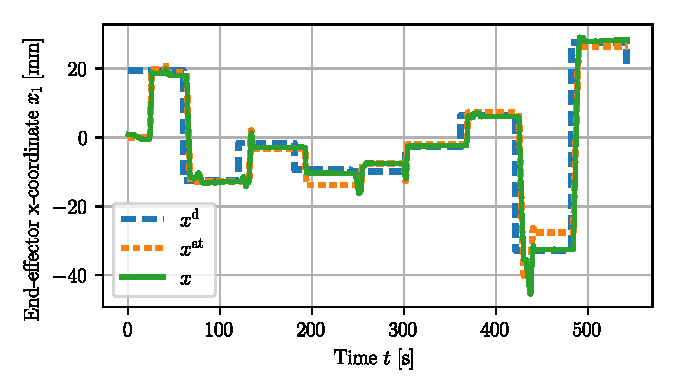
\includegraphics[width=0.47\textwidth, trim={5, 5, 5, 5}]{braincontrol/figures/setpoint_regulation/20231031_181745_pee_x.pdf}\label{fig:braincontrol:experimental_results:setpoint_regulation:keyboard:pee_x}}
%     \subfigure[End-effector y-coordinate]{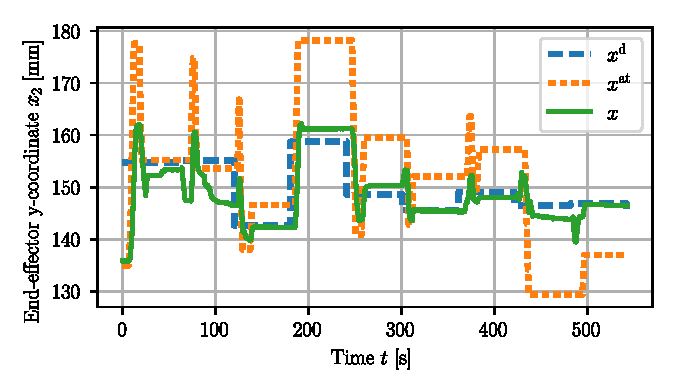
\includegraphics[width=0.47\textwidth, trim={5, 5, 5, 5}]{braincontrol/figures/setpoint_regulation/20231031_181745_pee_y.pdf}\label{fig:braincontrol:experimental_results:setpoint_regulation:keyboard:pee_y}}\\
%     \subfigure[Configuration $q$]{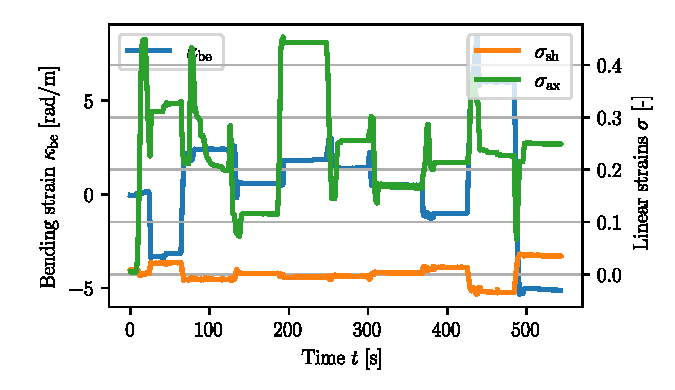
\includegraphics[width=0.47\textwidth, trim={5, 5, 5, 5}]{braincontrol/figures/setpoint_regulation/20231031_181745_q.pdf}\label{fig:braincontrol:experimental_results:setpoint_regulation:keyboard:q}}
%     \subfigure[Control input $\phi$]{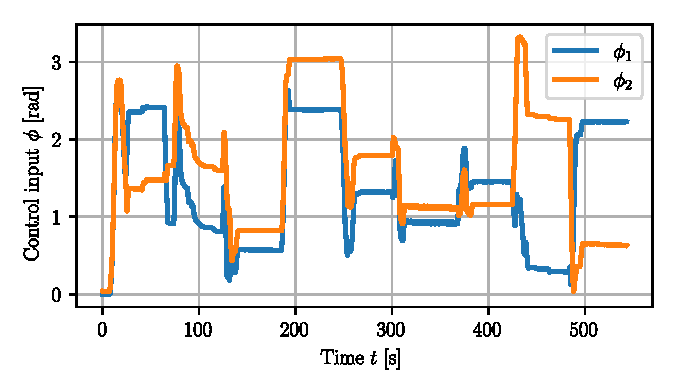
\includegraphics[width=0.47\textwidth, trim={5, 5, 5, 5}]{braincontrol/figures/setpoint_regulation/20231031_181745_phi.pdf}\label{fig:braincontrol:experimental_results:setpoint_regulation:keyboard:phi}}
%     \caption{Experimental results for tracking a reference trajectory of nine step functions with keyboard inputs. \textbf{Panel (a) \& (b):} The x/y-coordinate of the end-effector position with the solid line denoting the actual position, the dotted line the attractor position, and the dashed line the reference (i.e., the setpoint).
%     \textbf{Panel (c):} The evolution of the configuration.
%     \textbf{Panel(d):} The saturated planar control inputs. }\label{fig:braincontrol:experimental_results:setpoint_regulation:keyboard}
% \end{figure*}

\begin{figure*}[t]
    \centering
    \subfigure[End-effector x-coordinate]{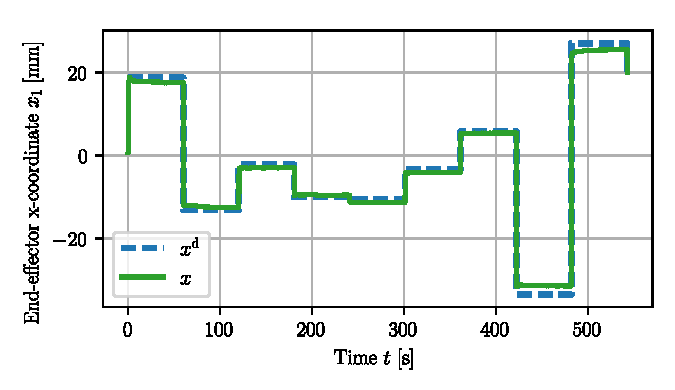
\includegraphics[width=0.47\textwidth, trim={5, 5, 5, 5}]{braincontrol/figures/setpoint_regulation/20231030_181558_pee_x.pdf}\label{fig:braincontrol:experimental_results:setpoint_regulation:computational:pee_x}}
    \subfigure[End-effector y-coordinate]{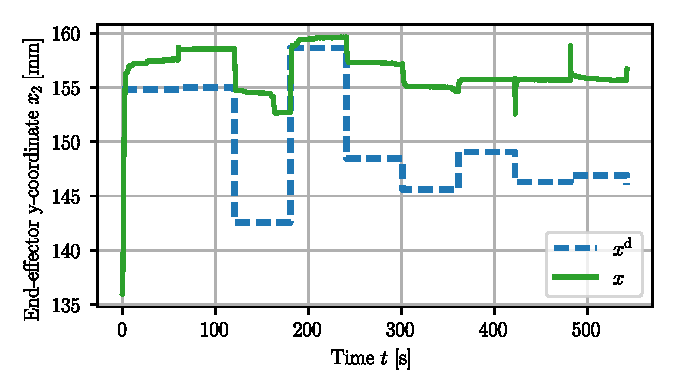
\includegraphics[width=0.47\textwidth, trim={5, 5, 5, 5}]{braincontrol/figures/setpoint_regulation/20231030_181558_pee_y.pdf}\label{fig:braincontrol:experimental_results:setpoint_regulation:computational:pee_y}}\\
    \subfigure[Configuration $q$]{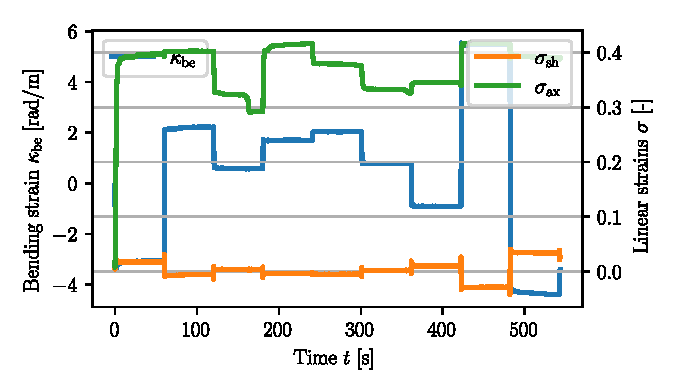
\includegraphics[width=0.47\textwidth, trim={5, 5, 5, 5}]{braincontrol/figures/setpoint_regulation/20231030_181558_q.pdf}\label{fig:braincontrol:experimental_results:setpoint_regulation:computational:q}}
    \subfigure[Control input $\phi$]{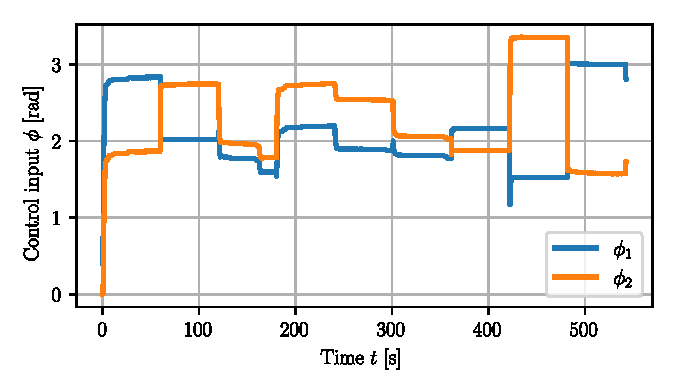
\includegraphics[width=0.47\textwidth, trim={5, 5, 5, 5}]{braincontrol/figures/setpoint_regulation/20231030_181558_phi.pdf}\label{fig:braincontrol:experimental_results:setpoint_regulation:computational:phi}}
    \caption{Experimental results for tracking a reference trajectory of nine step functions directly with the Cartesian impedance controller with access to the privileged information $x^\mathrm{d}$. \textbf{Panel (a) \& (b):} The x/y-coordinate of the end-effector position with the solid line denoting the actual position, the dotted line the attractor position, and the dashed line the reference (i.e., the setpoint).
    \textbf{Panel (c):} The evolution of the configuration.
    \textbf{Panel(d):} The saturated planar control inputs. }\label{fig:braincontrol:experimental_results:setpoint_regulation:computational}
\end{figure*}


\subsubsection{Online robot control}
Now, the participant operates the HSA robot in real time, with both classifiers being executed online.
Moreover, we map the outputs of the classifier into actionable commands: we initialize the x-axis as the active axis of movement (i.e., $e_\mathrm{a} = [1,0]$). When the first classifier detects jaw clenching for at least \SI{80}{\percent} of samples over a duration of \SI{2.8}{s}, we switch to the y-axis: $e_\mathrm{a} = [0,1]$ and vice-versa. If we do not detect any jaw clenching artifacts, we evaluate the output of the second classifier in parallel: if there is motor imagery activity identified in the \gls{EEG} classifier, the attractor will be moved in the positive direction (i.e., $s=1$) along $e_\mathrm{a}$. In contrast, if the \gls{EEG} signals are classified as the participant being at rest, $s=-1$ (i.e., movement in the negative direction).

% ~\footnote{\url{https://www.neuroconcise.co.uk/}}.

\subsection{Setpoint regulation}\label{sub:braincontrol:experiments:setpoint_regulation}
We randomly generate nine setpoints $x^\mathrm{d}(t) \in \mathbb{R}^2$ within the operational workspace of the robot (see Fig.~\ref{fig:braincontrol:hsa_workspace} and display them as a red circle to the user over a duration of \SI{540}{s}.
The user can freely move the attractor to reach and keep the end-effector at the setpoint.
% In addition to the motor imagery-based control, we conduct experiments where the subject controls the robot with a keyboard.
% As a keyboard is a very efficient and precise \gls{HMI}~\textcolor{red}{TODO Sonal: add a citation if you can find one}, this represents an upper bound on the performance we could expect from the \gls{BCI}.
% Here, the space button is used to switch that axis of movement $e_\mathrm{a}$ and positive/negative movement can be controlled via the left/right arrows.
Furthermore, we execute an experiment in which the computational controller has access to normally privileged information: as we substitute $x^\mathrm{at}$ with $x^\mathrm{d}$ in \eqref{eq:braincontrol:cartesian_impedance_controller}, the Cartesian impedance controller now immediately regulates the robot towards the setpoint.
By excluding the \gls{BMI} from the pipeline, this provides us with a reference of the performance we can expect from the computational controller and, with that, also represents a performance upper bound.

% sequence of stills with 10 images
\begin{figure*}[tb]
    \centering
    \subfigure[$t=\SI{0}{s}$]{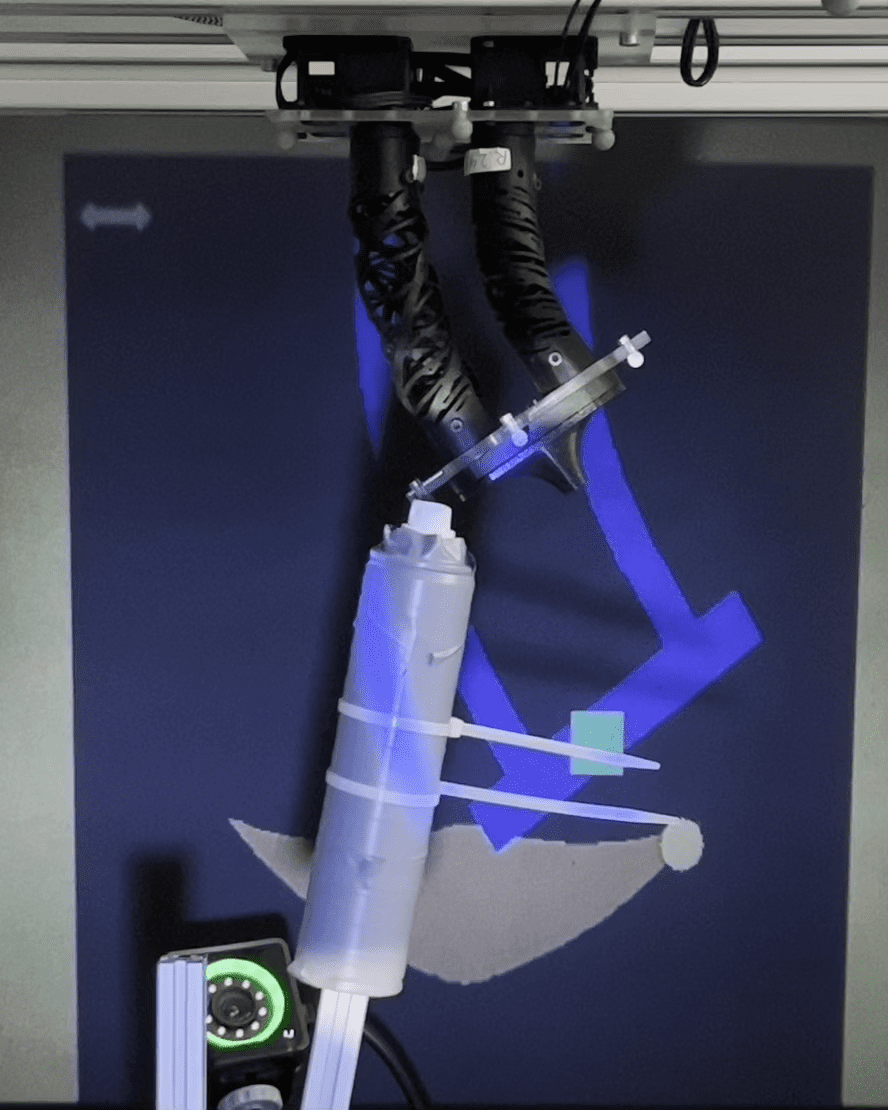
\includegraphics[width=0.192\textwidth]{braincontrol/figures/adl_task/20231031_203004_trimmed_and_cropped-0001-min.png}}
    \subfigure[$t=\SI{12}{s}$]{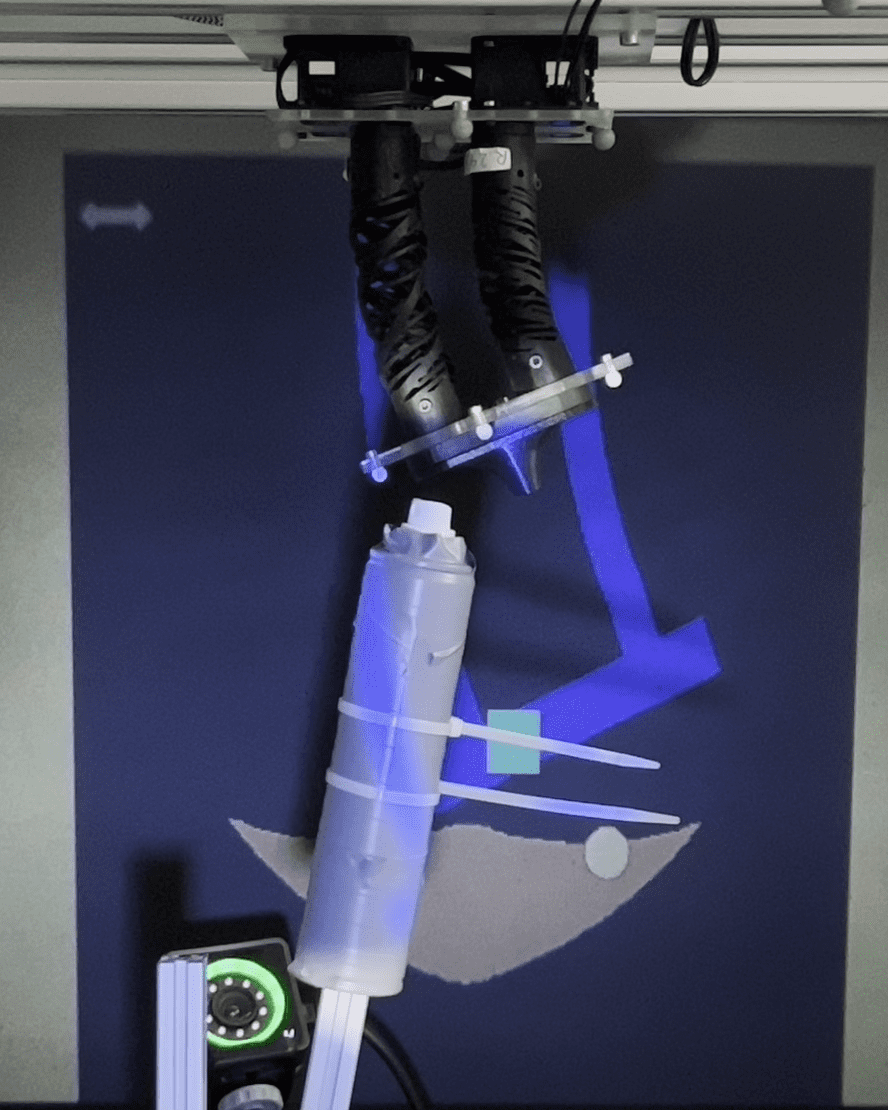
\includegraphics[width=0.192\textwidth]{braincontrol/figures/adl_task/20231031_203004_trimmed_and_cropped-0002-min.png}}
    \subfigure[$t=\SI{24}{s}$]{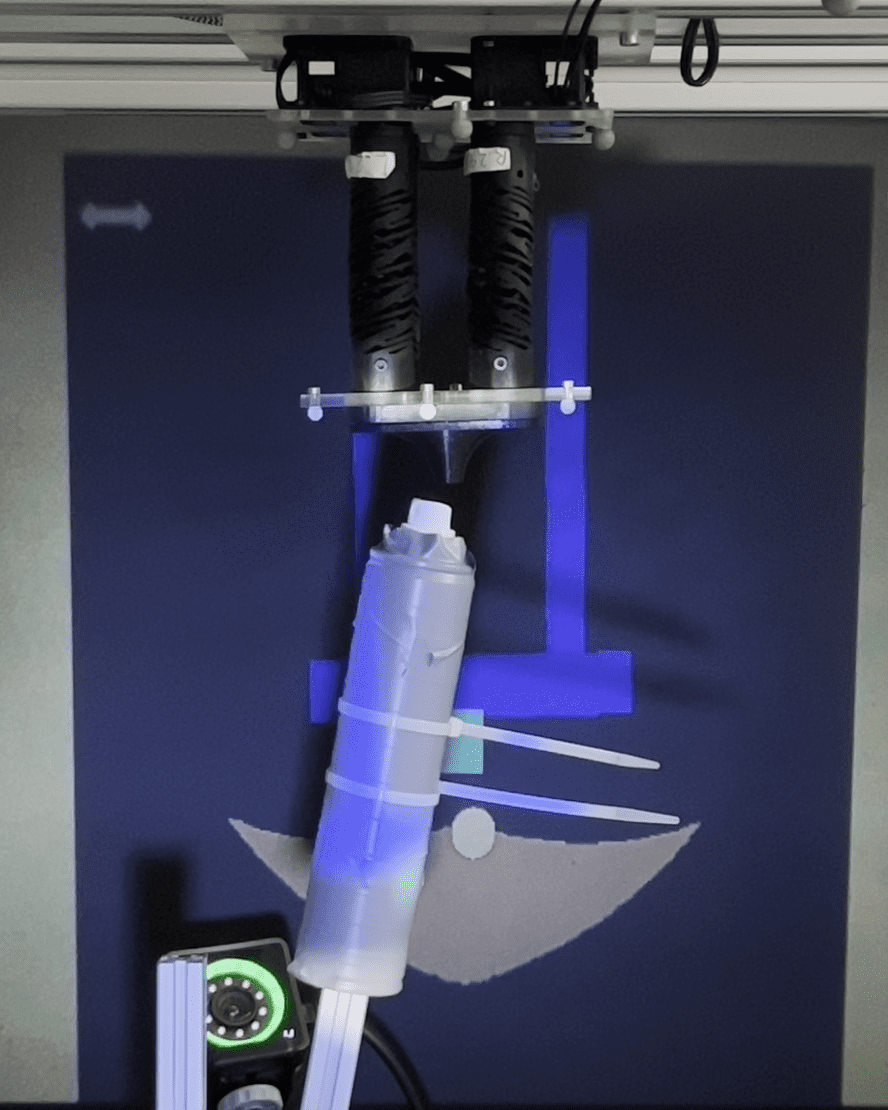
\includegraphics[width=0.192\textwidth]{braincontrol/figures/adl_task/20231031_203004_trimmed_and_cropped-0003-min.png}}
    \subfigure[$t=\SI{36}{s}$]{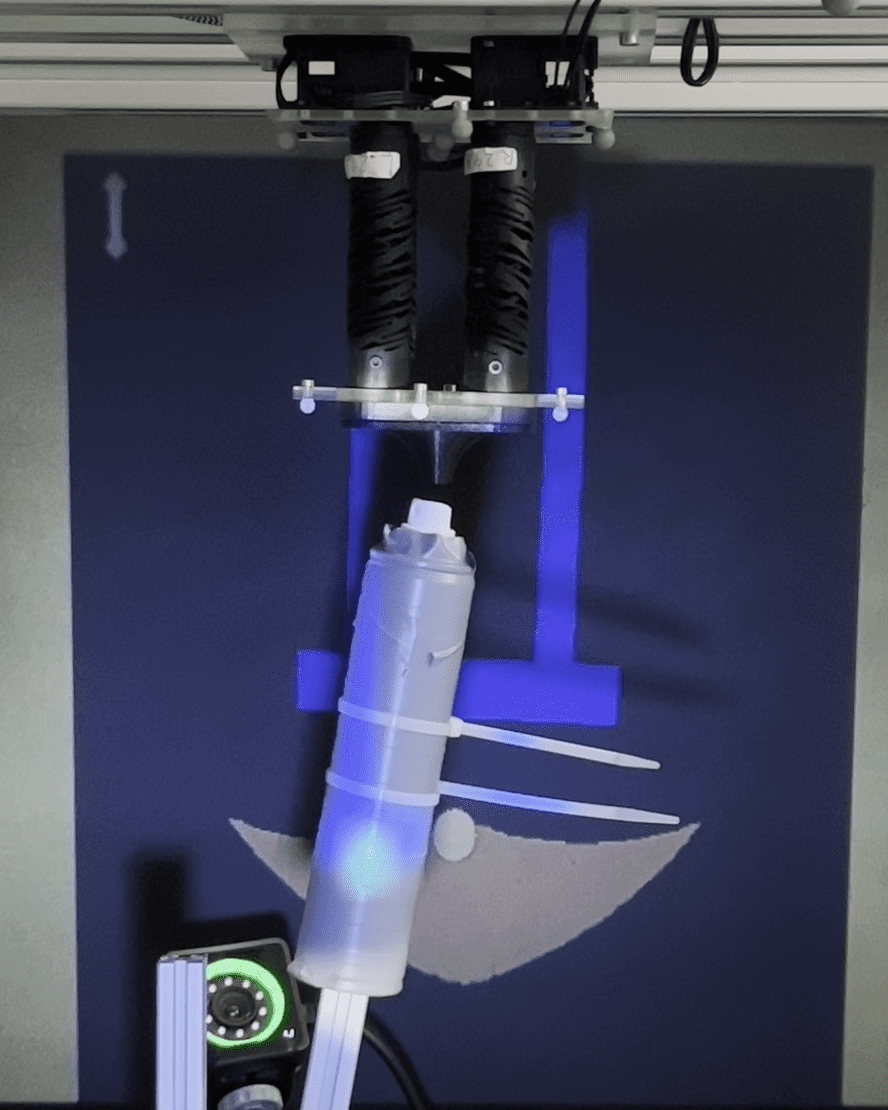
\includegraphics[width=0.192\textwidth]{braincontrol/figures/adl_task/20231031_203004_trimmed_and_cropped-0004-min.png}}
    \subfigure[$t=\SI{48}{s}$]{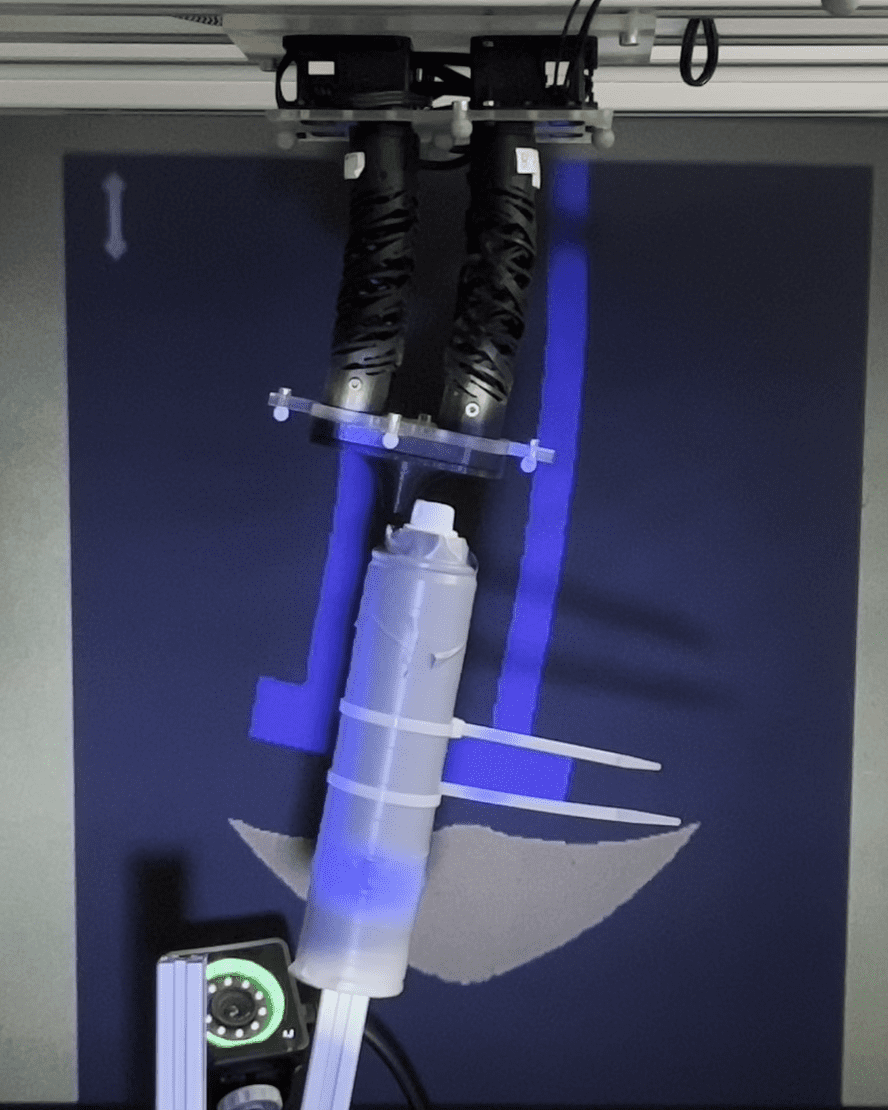
\includegraphics[width=0.192\textwidth]{braincontrol/figures/adl_task/20231031_203004_trimmed_and_cropped-0005-min.png}}\\
    \subfigure[$t=\SI{60}{s}$]{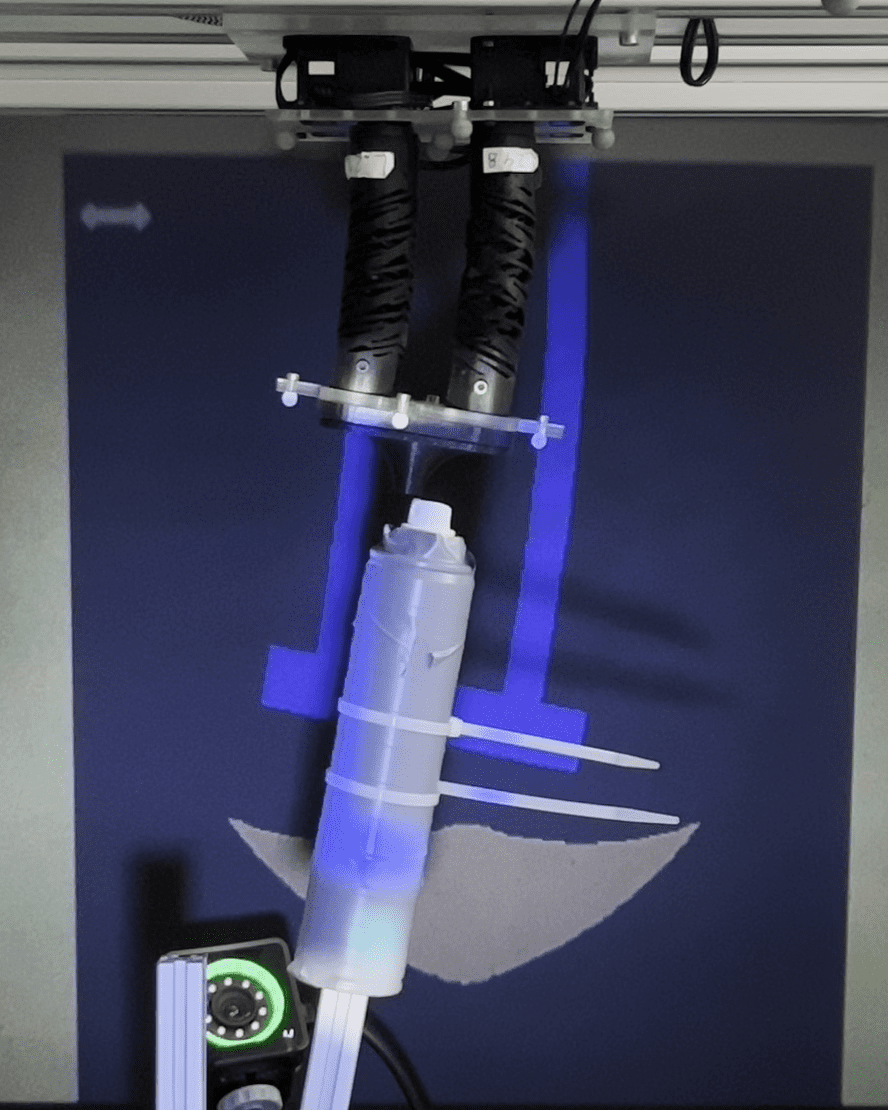
\includegraphics[width=0.192\textwidth]{braincontrol/figures/adl_task/20231031_203004_trimmed_and_cropped-0006-min.png}}
    \subfigure[$t=\SI{72}{s}$]{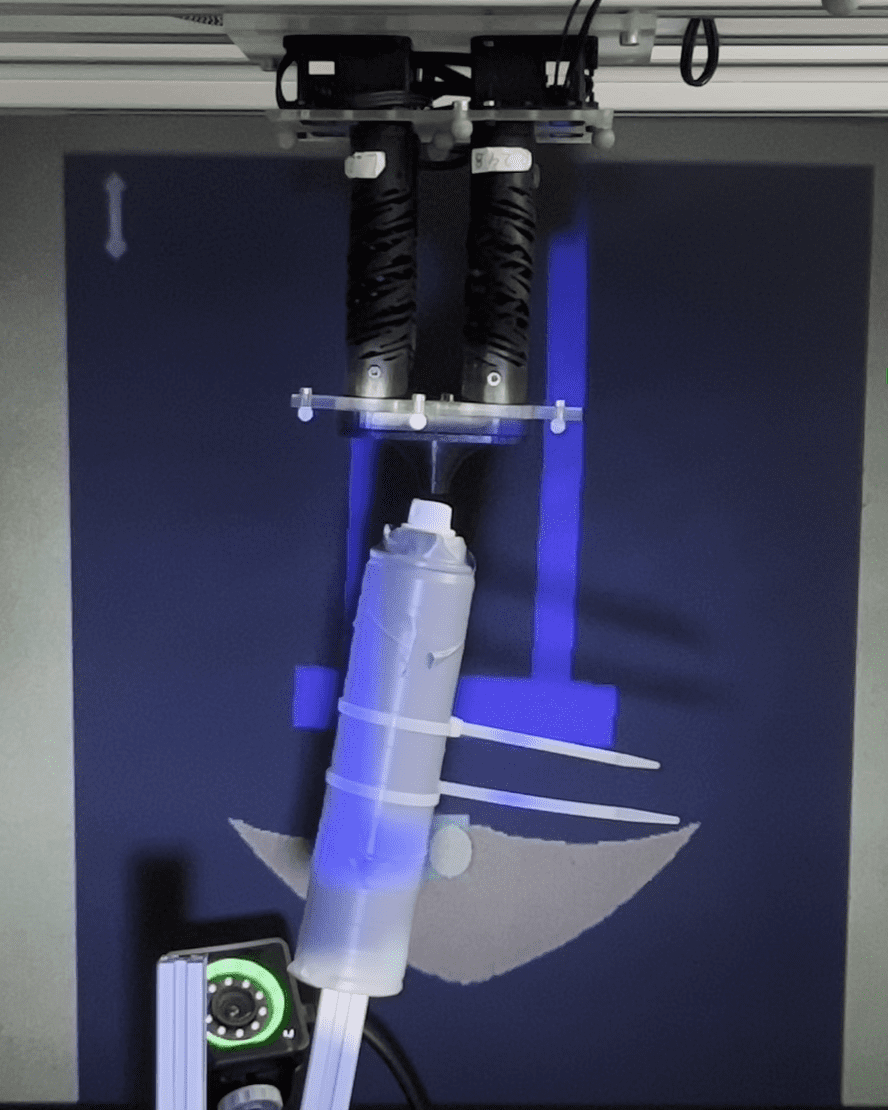
\includegraphics[width=0.192\textwidth]{braincontrol/figures/adl_task/20231031_203004_trimmed_and_cropped-0007-min.png}}
    \subfigure[$t=\SI{84}{s}$]{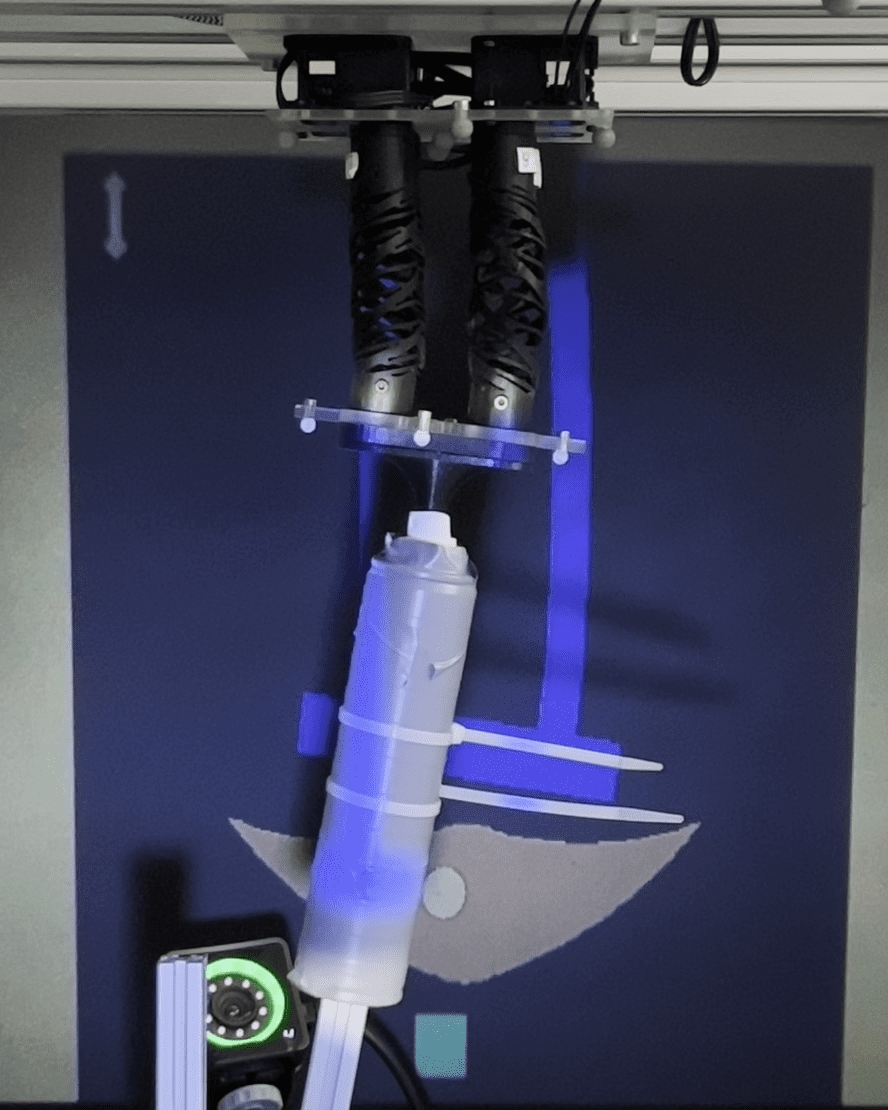
\includegraphics[width=0.192\textwidth]{braincontrol/figures/adl_task/20231031_203004_trimmed_and_cropped-0008-min.png}}
    \subfigure[$t=\SI{96}{s}$]{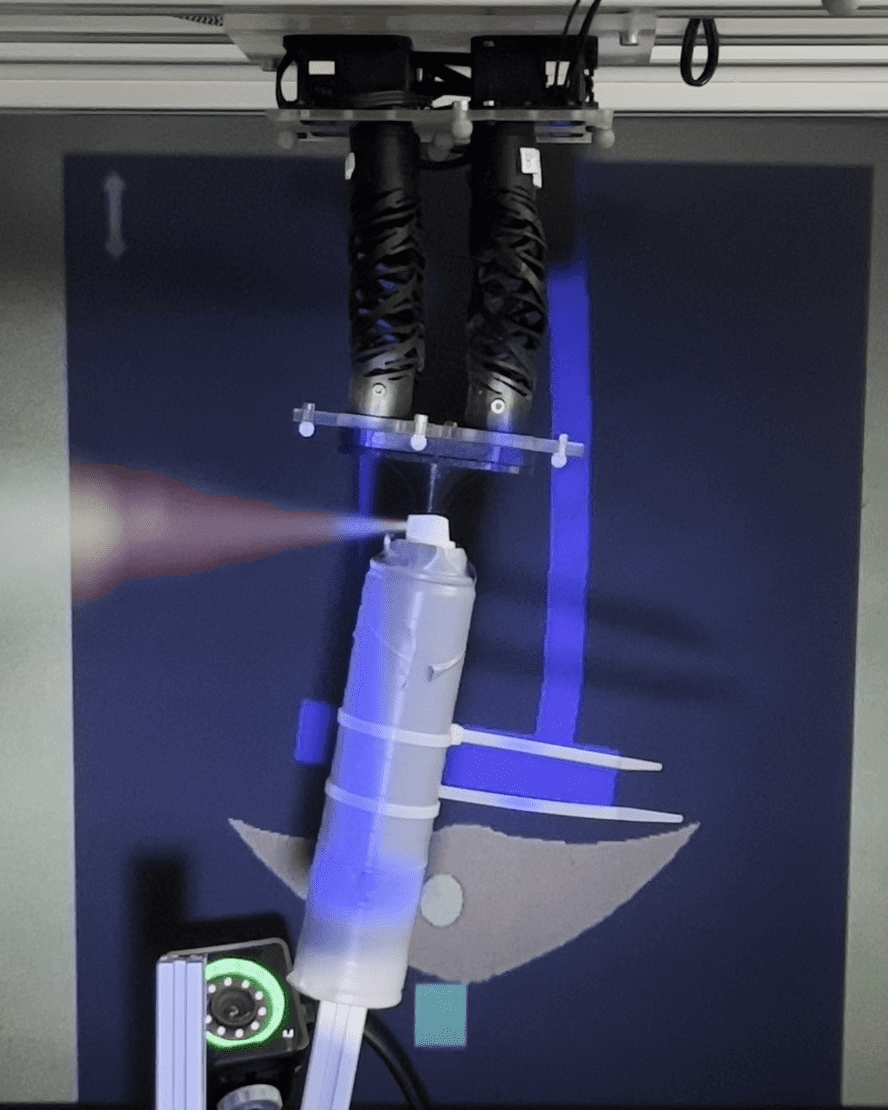
\includegraphics[width=0.192\textwidth]{braincontrol/figures/adl_task/20231031_203004_trimmed_and_cropped-0009_edited-min.png}\label{fig:braincontrol:experimental_results:adl_task_sequence_of_stills:spraying}}
    \subfigure[$t=\SI{108}{s}$]{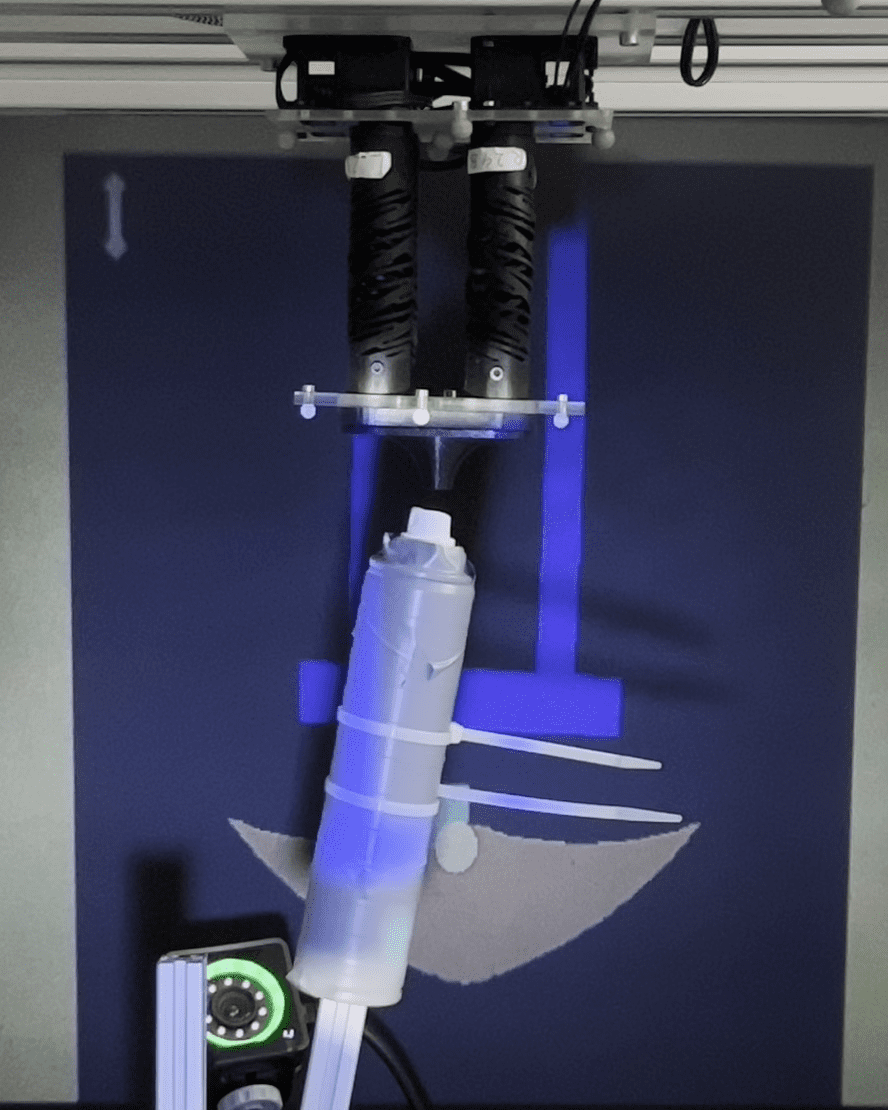
\includegraphics[width=0.192\textwidth]{braincontrol/figures/adl_task/20231031_203004_trimmed_and_cropped-0010-min.png}}
    \caption{Sequence of stills for completing a basic Activity of Daily Living (ADL) by controlling the robot with EEG-based motor imagery.
    \emph{Note: }Fig.~\ref{fig:braincontrol:experimental_results:adl_task_sequence_of_stills:spraying} is edited for improved contrast.
    }\label{fig:braincontrol:experimental_results:adl_task:sequence_of_stills}
\end{figure*}

\subsection{Interacting with the environment on a real-world task}\label{sub:braincontrol:experiments:adl}
We consider the \gls{ADL} task of releasing hairspray by actuating the button of its container with the \gls{HSA} robot's end-effector. For successful execution, the end-effector must be very stiff in the normal direction of the contact. On the other hand, we might want to benefit from the physical intelligence of the system by being relatively flexible in the tangential direction. Therefore, we first define the perpendicular stiffness $k_\perp = \SI{500}{N\per\meter}$ and the tangential stiffness as $k_\parallel = \SI{50}{N \per \meter}$. We assume that the normal direction of the contact can be described by the polar angle $\theta_\perp$ (with respect to the x-axis). We envision that in the future, the user can adjust such stiffness characteristics online via a \gls{BMI} system similar to~\cite{schiatti2017soft}. In this work, however, we estimate by visual inspection that $\theta_\perp=\SI{1.31}{rad}$.
The Cartesian stiffness matrix in global coordinates is then given by $K_x = R(\theta_\perp) \, \mathrm{diag}(k_\perp, k_\parallel) \, R(\theta_\perp)^\mathrm{T}$
where $R(\theta_\perp) \in SO(2)$ is the rotation matrix between global and contact frames.
% Analog to the setpoint regulation task, the user can move the attractor freely in Cartesian space when executing the described \gls{ADL} task.

\begin{figure*}[tb]
    \centering
    \subfigure[End-effector $x$-coordinate]{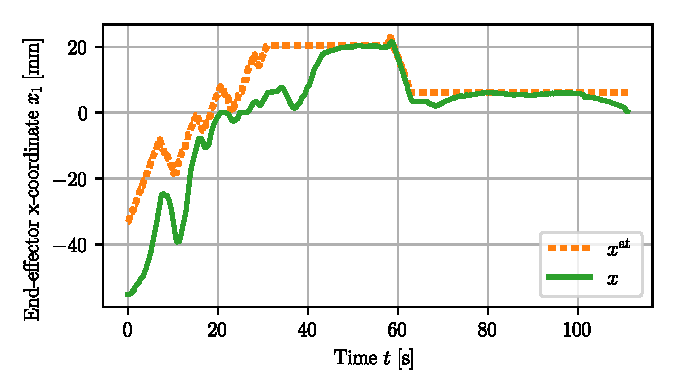
\includegraphics[width=0.47\textwidth, trim={5, 5, 5, 5}]{braincontrol/figures/adl_task/20231031_203004_pee_x.pdf}\label{fig:braincontrol:experimental_results:adl_task:brain:pee_x}}
    \subfigure[End-effector $y$-coordinate]{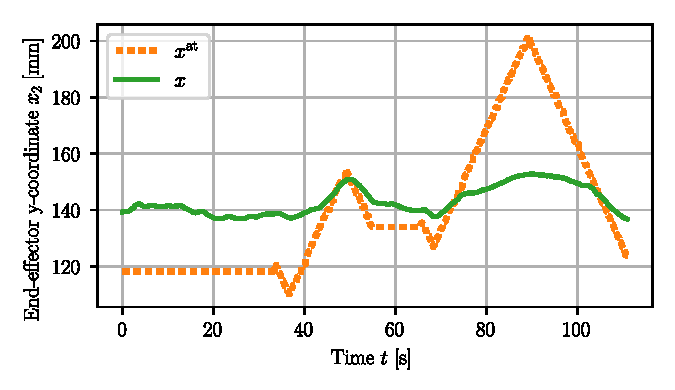
\includegraphics[width=0.47\textwidth, trim={5, 5, 5, 5}]{braincontrol/figures/adl_task/20231031_203004_pee_y.pdf}\label{fig:braincontrol:experimental_results:adl_task:brain:pee_y}}
    \\
    \subfigure[Configuration $q$]{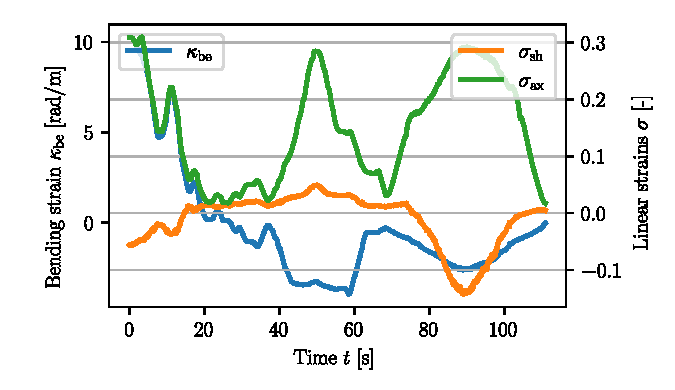
\includegraphics[width=0.47\textwidth, trim={5, 5, 5, 5}]{braincontrol/figures/adl_task/20231031_203004_q.pdf}\label{fig:braincontrol:experimental_results:adl_task:brain:q}}
    % \subfigure[Joy signal $u$]{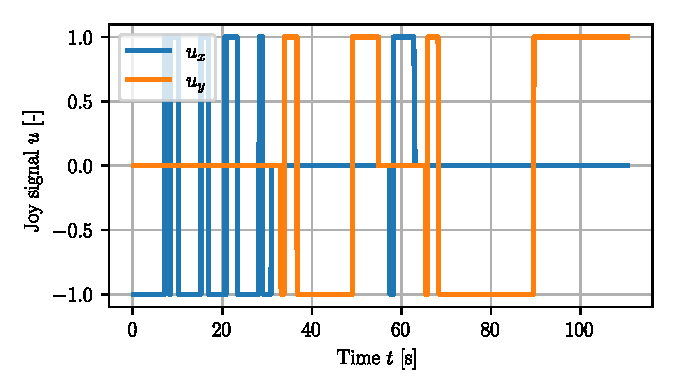
\includegraphics[width=0.49\textwidth, trim={5, 5, 5, 5}]{braincontrol/figures/adl_task/20231031_203004_joy_signal.pdf}\label{fig:braincontrol:experimental_results:adl_task:brain:u}}
    \subfigure[Control input $\phi$]{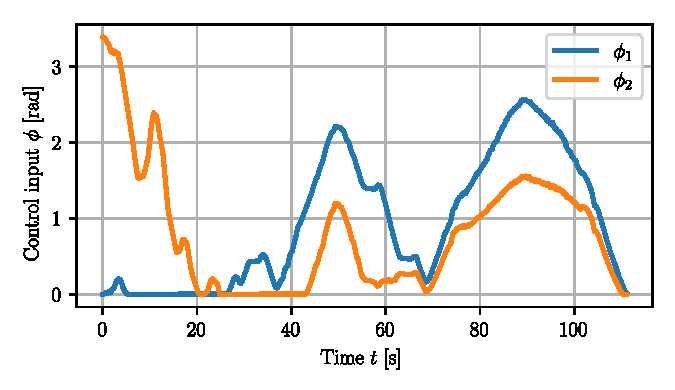
\includegraphics[width=0.47\textwidth, trim={5, 5, 5, 5}]{braincontrol/figures/adl_task/20231031_203004_phi.pdf}\label{fig:braincontrol:experimental_results:adl_task:brain:phi}}
    \caption{Experimental results for completing a basic Activity of Daily Living (ADL) by controlling the robot with EEG-based motor imagery. \textbf{Panel (a) \& (b):} The x/y-coordinate of the end-effector with the solid line and dotted lines denoting the actual and attractor position, respectively.
    \textbf{Panel (c):} The evolution of the configuration.
    % \textbf{Panel (c):} The joy commands $u$ derived from the classified brain signals used to move the attractor in Cartesian space.
    \textbf{Panel(d):} The saturated planar control inputs. }\label{fig:braincontrol:experimental_results:adl_task:brain}
\end{figure*}

\subsection{Evaluation metrics}
% Look at this paper for evaluation metrics: ~\cite{rakshit2020hybrid}
In the following, we will introduce and define a few metrics that help us assess the performance of the approach.

\subsubsection{Event-Related Synchronization/De-Synchronization:}
We apply \gls{ERD} / \gls{ERS}~\cite{pfurtscheller1999event} to demonstrate the difference between \gls{EEG} signals when the participant imagines right-hand movement vs. rest, i.e., no activity. \gls{ERD}/\gls{ERS} corresponds to a shift in power during imagination with respect to a baseline. It is defined by
\begin{equation}
    \mathrm{ERD/ERS}(t, f) = \frac{P(t, f) - P_{\mathrm{base}}(f)}{P_{\mathrm{base}}(f)},
\end{equation}
where $\mathrm{ERD/ERS}(t, f)$ represents the \gls{ERD} or \gls{ERS} at a specific time $t$ and frequency $f$, $P(t, f)$ stands for the power of brain activity during imagination, and $P_\mathrm{base}(f)$ denotes the baseline power. 

\subsection{Step response metrics}
For the task of setpoint regulation, we analyze primarily two aspects: (a) is the participant able to reach the proximity of setpoint within the (generously) allotted time of \SI{60}{s}? We define the proximity of the setpoints as $\lVert x^\mathrm{d} - x(t)\rVert_2 \leq \SI{2}{mm}$. And (b) what is the response time for reaching for the first time the proximity of the setpoint?